%!TEX root = /Users/ede/Documents/Master/19_AS/Ausarbeitung/as-ausarbeitung.tex
\section{Evaluation der vorgestellten Verfahren} % (fold)
\label{sec:evaluation_der_verfahren}

In diesem Kapitel erfolgt die Darstellung der Ergebnisse der jeweils von den Autoren vorgenommenen Evaluation der eingesetzten Verfahren. Dabei sollen unterschiedliche Perspektiven beleuchtet werden. Der Aufbau des Evaluationsszenarios bestimmt die Ergebnisse. Insofern soll beschrieben werden, welche Auswahl an Photos und Tags für die Evaluation verwendet wurden und ob diese nach speziellen Kriterien ausgesucht wurden. Die Art und Weise der Evaluation ist ebenfalls von Bedeutung, wobei hier zwischen automatischer und manueller bzw. durch Menschen durchgeführte Messungen der Verfahren unterschieden wird. Die Auswahl der Referenzdaten entscheidet zu welcher Basis die Verbesserungen gemessen werden und die Auswahl der Metriken entscheidet, was überhaupt gemessen wird und ob basierend darauf eine fundierte Entscheidungen über die Qualität der Verfahren getroffen werden kann. Ebenso sollte auch die Leistung und Skalierbarkeit der Algorithmen von den Autoren untersucht werden, da zum Beispiel der Einsatz solch eines Systems bei Flickr stark von der Performanz abhängt und auch für viele Milliarden von Photos und Tags funktionieren muss. Schließlich sollen die Ergebnisse der Evaluation selbst präsentiert werden.

% - aufbau des evaluationsszenarios (welche auswahl an photos und tags wurde vorgenommen,)
% - art und weise der evaluation (automatisch, manuell, was sind die referenzdaten, wie wird die qualität bewertet), welche metriken werden angewandt
% - performance der algorithmen(gibts es laufzeit analysen der algorithmen, lässt sich das verfahren skalieren)
% - qualität der ergebnisse (sind verbesserung durch das Ranking entstanden, welche methode/kombination von methoden weist das beste ranking)
% - vergleichbarkeit der ergebnisse(in wie weit ist die evaluation standardisiert, welchen mehrwert/errungenschaften hat die arbeit hervorgebracht)

\subsection{Ergebnisse der Evaluation von Sigurbjörnsson und van Zwol} % (fold)
\label{sub:ergebnisse_der_evaluation_von_collectiveknowledge}

Die Autoren von \cite{collectiveKnowledge}, Sigurbjörnsson und van Zwol, untersuchen die in Kapitel \ref{sub:ranking_basierend_auf_kollektivem_wissen_nach_zwol} vorgestellten Methoden auf ihre Leistung hin, möglichst relevante Tags zu den bereits vergebenen, benutzerdefinierten Tags vorzuschlagen. Dabei werden die eingesetzten Strategien einzeln betrachtet und evaluiert. Tabelle \ref{tab:fourStrategiesBjoern} veranschaulicht die vier untersuchten Kombinationen.

\begin{table}[htbp]
  \centering
  \begin{tabular}{c|cc}
    \hline
     & \textbf{vote} & \textbf{sum}\\
    \hline
    \textbf{no-promotion} & vote & sum\\
    \hline
    \textbf{promotion} & vote\textsuperscript{+} & sum\textsuperscript{+}\\
    \hline
  \end{tabular}
  \caption{Die vier Kombinationen von Aggregations- und Promotionsalgorithmen nach \cite{collectiveKnowledge}}
  \label{tab:fourStrategiesBjoern}
\end{table}


Die Autoren bewerten, wie das System auf unterschiedliche Anzahl bereits vorhandener Tags reagiert. Weiterhin wird untersucht, ob das Verfahren für die WordNet Kategorien aus Abbildung \ref{fig:collectiveKnowledge_word_net_categories}, Kapitel \ref{ssub:tags} unterschiedliche gute Ergebnisse liefert. Das Hauptziel ist jedoch, dass die vorgeschlagenen Tags möglichst nach ihrer Relevanz zu dem Photo sortiert sind und irrelevante Tags nicht in dieser Liste vorkommen.

\subsubsection{Aufbau des Evaluationsszenarios} % (fold)
\label{ssub:aufbau_des_evaluationsszenarios}

Die an das Tag Ranking System gestellte Aufgabe bestand also darin, zu einem Photo mit bereits vorhandenen benutzerdefinierten Tags weitere, relevante Tags vorzuschlagen. Zu diesem Zweck wurden 331 Photos zufällig aus dem Bestand von Flickr gewählt, die jedoch aus mehrere begrenzten Sachgebieten stammten, in denen die Probanden, die die Relevanz der vorgeschlagenen Tags bewerteten, sich auskennen.
Weiterhin stellten die Autoren sicher, dass die Photos möglichst gleichmäßig auf die in Kapitel \ref{sub:klassifikation_von_tags} vorgestellten Klassen aus Tabelle \ref{tab:classes_for_tags_collective} verteilt sind. Dadurch sollte überprüft werden, ob das Verfahren sich je nach Anzahl der bereits vergebenen Tags unterschiedlich verhält bzw. unterschiedlich gute Ergebnisse liefert.
  
131 dieser Photos wurden für das manuelle Training der im Algorithmus benötigten Parameter $m,	k_r,	k_s, k_d $ verwendet. Die Werte sind in Tabelle \ref{tab:optimalParameterBjoern} aufgeführt. Die restlichen 200 Photos dienten als Grundlage für die Evaluation. Dabei sollten die Probanden jedes Photo und die vom System vorgeschlagenen Tags betrachten und für die ersten 10 Tags jeweils die Beschreibbarkeit bzw. Relevanz des Tags für das Photo auf einer Skala von eins bis vier (\emph{sehr gut, gut, nicht gut, weiß nicht}) bewerten. Gleichzeitig wurden den Probanden weitere Kontextinformationen zum Photo wie Titel, Beschreibung, Aufnahmedatum usw. präsentiert, so dass diese eine möglichst fundierte Bewertung abgeben können. Die Option \emph{weiß nicht} bestand für den Fall, dass doch nicht genug Wissen für eine begründete Bewertung vorhanden war. In der Auswertung wurden die Wahlmöglichkeiten \emph{sehr gut} und \emph{gut} zu einem Wert zusammen gefasst, um eine einfachere Auswertung im Sinne von \emph{relevant} und \emph{nicht relevant} durchführen zu können.
  
\begin{table}[htbp]
  \centering
  \begin{tabular}{ccccc}
    \hline
     & \textbf{m} & \textbf{k\textsubscript{s}} & \textbf{k\textsubscript{d}} & \textbf{k\textsubscript{r}}\\
    \hline                          
    \textbf{sum} & 10 & - & - & -\\
    \hline                          
    \textbf{vote} & 10 & - & - & -\\
    \hline                          
    \textbf{sum\textsuperscript{+}} & 25 & 0 & 12 & 3\\
    \hline                          
    \textbf{vote\textsuperscript{+}} & 25 & 9 & 11 & 4\\
    \hline
  \end{tabular}
  \caption{Die optimalen Parameterwerte für $m,	k_r,	k_s, k_d$ aus \cite{collectiveKnowledge}.}
  \label{tab:optimalParameterBjoern}
\end{table}


% subsubsection aufbau_des_evaluationsszenarios (end)

\subsubsection{Metriken} % (fold)
\label{ssub:metriken}
Sigurbjörnsson und van Zwol stellen in \cite{collectiveKnowledge} drei unterschiedlich ausgerichtete Metriken zum Bewerten des Verfahrens auf. Diese sind vor allem auf die qualitativen Aspekte von Tag Ranking ausgerichtet und werden manuell, sprich durch Probandenbefragung ermittelt.
\begin{itemize}
  \item \textbf{Mean Reciprocal Rank (MRR)} misst die Position des ersten relevanten Tags in der Vorschlagsliste, gemittelt über alle bewerteten Photos. Dieser Wert sagt aus, wie gut das System in der Lage ist, die relevantesten Tags an vorderster Stelle zu positionieren.
  \item \textbf{Success at rank k (S@k)} protokolliert die Wahrscheinlichkeit, innerhalb der ersten $k$ Elemente der Vorschlagsliste relevante Tags vom System zu erhalten. Dieser Wert wird für $k = 1$ und $k = 5$ ermittelt.
  \item \textbf{Precision at rank k (P@k)} erfasst die Relation bzw. Anteil von relevanten zu irrelevanten vorgeschlagenen Tags. Dieser Wert wird ebenfalls über alle Photos gemittelt und erfasst die ersten 5 vorgeschlagenen Tags.
\end{itemize}

Als Referenzdaten wird angenommen, dass gar kein Ranking von Tags statt finden, womit klar ist, dass die Algorithmen eine grundsätzliche Verbesserung darstellen.

% subsubsection metriken (end)

\subsubsection{Ergebnisse der Evaluation} % (fold)
\label{ssub:ergebnisse_der_evaluation}

Die Ergebnisse sind in die vier Bereiche Aggregationsstrategien, Promotion, Photo Klassen und Semantisch Analyse aufgeteilt und werden im Folgenden gesondert beschrieben. Die Tabelle \ref{tab:strategiesrResultsBjoern} enthält die Ergebnisse der von \cite{collectiveKnowledge} durchgeführten Evaluation. 

\begin{table}[htbp]
  \centering
  \begin{tabular}{ccccc}
  \hline
   & \textbf{MRR} & \textbf{S@1} & \textbf{S@5} & \textbf{P@5}\\
  \hline
  Basisstrategien\\
  \textbf{sum} & .7628 & .6550 & .9200 & .4930\\
  \textbf{vote} & .6755 & .4550 & .8750 & .4730\\
  \hline
  Promototionsstrategien\\
  \textbf{sum\textsuperscript{+}} & .7718 & .6600 & .9450 & .5080\\
  \textbf{vote\textsuperscript{+}} & .7883 & .6750 & .9400 & .5420\\
  \hline
  Verbesserung durch Promotion\\
  \textbf{vote\textsuperscript{+} vs. sum} & 4.3\% & 3.1\% & 2.2\% & 9.9\%\\
  \hline
  \end{tabular}
  \caption{Die Ergebnisse der Evaluation aus \cite{collectiveKnowledge} für die Aggregation und Promotion. Die Werte geben in Prozenten die erfolgreichen, d.h. für gut oder sehr gut befundenen Ergebnisse an.}
  \label{tab:strategiesrResultsBjoern}
\end{table}

Bei der Betrachtung der zwei unterschiedlichen Aggregationsstrategien fällt auf, dass die \emph{summing strategy} bessere Ergebnisse liefert und dabei 65 Prozent aller Tags auf Position eins relevant sind. Innerhalb der ersten fünf vorgeschlagenen Tags sind in 92 Prozent der Fälle relevante Tags enthalten, wobei die Präzision bzw. der P@5 Wert aussagt, dass knapp die Hälfte der fünf ersten vorgeschlagenen Tags nicht relevant sind. Damit ist belegt, dass durch die summing Strategie der Annotationsprozess für den Benutzer verbessert werde konnte, da nun relevante Tags vorgeschlagenen werden. Gleichzeitig spricht dies für die Verwendung von co-occurence bei Tag Ranking Verfahren, da dies in der summing Strategie eingesetzt wird.

Die Einsatz der Promotion von Tags, also das Abwerten sehr hochfrequenter und sehr niederfrequenter Tags, liefert im Vergleich zu den Basisstrategien für alle Metriken bessere Ergebnisse, wobei die voting Strategie etwas bessere Resultate liefert. Die summing Strategie erzielt in Kombination mit der Promotion von Tags leicht bessere Werte in der S@5 Metrik, die voting Strategie erzielt jedoch eine bessere Präzision, das heißt es sind mehr relevante Tags in der Vorschlagsliste enthalten. Insgesamt ist den Ergebnissen nach die voting Strategie in Kombination mit der Promotion die beste Variante. Die Promotion der Tags steigert die Leistung des Verfahrens signifikant, wie in der letzten Zeile der Tabelle \ref{tab:strategiesrResultsBjoern} zu entnehmen ist.
 
Bei der Betrachtung der Photo Klassen, die nach der Anzahl ihrer benutzerdefinierten Tags unterteilt sind (siehe Tabelle \ref{tab:classes_for_tags_collective}), und der Leistung des vorgestellten Verfahrens, zeigt sich, dass die besten Ergebnisse in der Klasse I und II erreicht werden. Auch hierbei fällt auf, dass die Promotion deutlich bessere Werte für die Metriken liefert, wobei diese bei mehr benutzerdefinierten Tags stärker ausfällt als bei nur geringer Anzahl vorgegebener Tags zu einem Photo. Die Auswertung für die Photo Klassen ist in dieser Ausarbeitung nicht enthalten und kann in \cite{collectiveKnowledge}, Tabelle 5 eingesehen werden.
%TODO: Tabelle 5 könnte noch rein, dann aber auch obigen letzten satz wieder entfernen

\begin{table}[htbp]
  \centering
  \begin{tabular}{lr}
  \hline
  \textbf{WordNet} & \textbf{Akzeptanzverhältnis}\\
  \hline
  Orte & 71\%\\
  \hline
  Artefakte oder Objekte & 61\%\\
  \hline
  Andere & 53\%\\
  \hline
  Handlungen oder Ereignisse & 51\%\\
  \hline
  Zeit & 46\%\\
  \hline
  Nicht klassifiziert & 39\%\\
  \hline
  Personen oder Gruppen & 33\%\\
  \hline
  \end{tabular}
  \caption{Der Bezug zwischen WordNet Kategorien und deren Akzeptanzverhältnis durch die Probanden aus \cite{collectiveKnowledge}.}
  \label{tab:wordNetResults}
\end{table}

Die semantische Analyse fokussiert auf die in Kapitel \ref{ssub:tags}, Abbildung \ref{fig:collectiveKnowledge_word_net_categories} ermittelten WordNet Kategorien für die Tags und erfasst, welche Kategorien von Tags eine bessere Akzeptanz bzw. Relevanzwerte durch die Probanden erfahren. So soll ermittelt werden, in welchen Kategorien von Begriffen das Verfahren bessere Ergebnisse liefert. Tabelle \ref{tab:wordNetResults} zeigt das Verhältnis von gut und sehr gut befundenen Tags zu den WordNet Kategorien. Ortsbezogene Tags wurden von den Probanden am meisten akzeptiert, gefolgt von Artefakten oder Objekten und Anderen. Personen, Gruppen und nicht klassifizierte Tags, die vom System vorgeschlagen werden, erreichen nur relativ schlechte Akzeptanzwerte. Damit eignet sich das Verfahren vornehmlich für die zuerst genannten Kategorien von Begriffen.

% subsubsection ergebnisse_der_evaluation (end)

\subsubsection*{Zusammenfassung} % (fold)
\label{ssub:zusammenfassung}
Die Ergebnisse der Evaluation sprechen eindeutig für den Einsatz von co-occurence basierten Verfahren für das Ranking von Tags. Die Auswertung hat ebenso gezeigt, dass auch die Analyse der bereits vorhanden Tags und das Einfließen dieser Analyse in Form von Promotion im Verfahren in einer verbesserten Leistung des Algorithmus resultiert.

Die Evaluation von Sigurbjörnsson und van Zwol bezieht sich jedoch nur auf die qualitativen Aspekten des Ranking Verfahrens. Quantitative Messungen zu Skalierbarkeit und Laufzeit wurden nicht durchgeführt. 
% subsubsection zusammenfassung (end)

% subsection ergebnisse_der_evaluation_von_collectiveknowledge (end)

\subsection{Ergebnisse der Evaluation von Liu u. a.} % (fold)
\label{sub:ergebnisse_der_evaluation_von_liu}

Ziel der Evaluation von Liu u. a. war die Erfolgsquote der beiden Hauptmethoden des Verfahrens, Initiale stochastische Schätzung des Tag Ranking Wertes und die Verbesserung des Tag Rankings durch einen Random Walk, im Einzelnen und in Kombination. Dazu wurden die Tags durch Probanden nach ihrer Relevanz zum zugehörigen Photo bewertet und anschließend mit Hilfe der NDCG Messung, die in Abschnitt \ref{ssub:metriken_liu} näher erläutert wird, evaluiert.

\subsubsection{Aufbau des Evaluationsszenarios} % (fold)
\label{ssub:aufbau_des_evaluationsszenarios_liu}
Um die Testdaten für die Evaluation zu sammeln, wurde zunächst eine Auswahl von zehn populären Tags aus Flickr getroffen. Für jeden Tag wurde eine Suche bei Flickr mit Begrenzung auf die ersten 5000 Photo durchgeführt, so dass eine Sammlung von 50.000 Testphotos inklusive der anhängenden Informationen wie Tags, Aufnahmezeit usw. aufgebaut wurde.

Auch in \cite{ranking} wurden die Testphotos und deren Tags einer Vorfilterung unterzogen. Dabei wurden Tags entfernt, die nicht im Thesaurus von Wikipedia enthalten waren. Dies ist damit begründet, dass viele Tags falsch geschriebene oder bedeutungslose Begriffe sind. Dadurch wurde die Menge von anfänglich mehr als 100.000 Tags auf 13.330 reduziert.

Aus der Gesamtmenge der Testphotos wurden daraufhin 10.000 Photos für die Evaluation eingesetzt. Fünf Probanden bewerteten die Tags aller Photos auf einer Skala von eins bis fünf, wobei folgende Wertungen abgegeben werden konnten: \emph{sehr relevant(5)}, \emph{relevant(4)}, \emph{teilweise relevant(3)}, \emph{schwach relevant(2)} und \emph{nicht relevant(1)}.
% subsubsection aufbau_des_evaluationsszenarios_liu (end)

\subsubsection{Metriken} % (fold)
\label{ssub:metriken_liu}

In \cite{ranking} wird zur Bewertung der Ergebnisse und vor allem deren Reihenfolge die \emph{Discounted cumulative gain}(DCG) Methode nach \cite{ndcg} verwendet. Diese Messmethode erfasst die Effektivität von Suchalgorithmen und verwandten Verfahren, wobei die Nützlichkeit (englisch: \emph{gain}) der einzelnen Elemente anhand ihrer Position in dem Suchergebnis und der Relevanz des Elementes gemessen wird. Als Vergleichsbasis der Messung dient eine Relevanzskala wie sie in Abschnitt \ref{ssub:aufbau_des_evaluationsszenarios_liu} beschrieben wurde. Der NDCG ist der \emph{normalized} DCG, welcher die Ergebnisse einer Messung auf einen Wert zwischen 0 und 1 normalisiert, so dass mehrere Suchanfrage miteinander verglichen werden können. Gleichung \ref{fig:ndcg} führt die Funktion zur Berechnung des NDCG für eine mit dem Verfahren gewertete Tag Liste $t_1, t_2, ..., t_n$ auf. $r(i)$ ist hierbei der Relevanzwert vom $i$-ten Tag und $Z_n$ ist die eben beschriebene Normalisierungskonstante.
\begin{figure}[hptb]
  \begin{equation}
  \label{fig:ndcg}
    N_n = Z_n \sum_{i=1}^n(2^{r(i)} - 1) / log(1+i)
  \end{equation}
\end{figure}

Nachdem für jede, gerankte Tag Liste eines Photos der NDCG ermittelt wurde, können die Werte gemittelt werden, so dass allgemeine Aussagen über alle Tags und Photos hinweg getroffen werden können. Je näher der NDCG Wert bei 1 liegt, desto relevanter sind die Ergebnisse in Bezug zum Suchwort. Im vorliegenden Fall wäre dies die Relevanz der Tags zum gezeigten Photo.
% subsubsection metriken_liu (end)

\subsubsection{Ergebnisse der Evaluation} % (fold)
\label{ssub:ergebnisse_der_evaluation_liu}

Obwohl Liu u. a. die Kombination von stochastischer Schätzung und Random Walk für das Berechnen von Tag Ranking Werte vorschlagen, haben Sie die beiden Methoden einzeln und in Kombination untersucht. Die Referenzwerte für die Evaluation wurden hierbei aus der originalen, von Flickr gelieferten Tag Liste bezogen. Die Ergebnisse der Messung der Verfahren mittels NDCG ist an Abbildung \ref{fig:images_ndcgAll} dargestellt.
\begin{figure}[htbp]
  \centering
    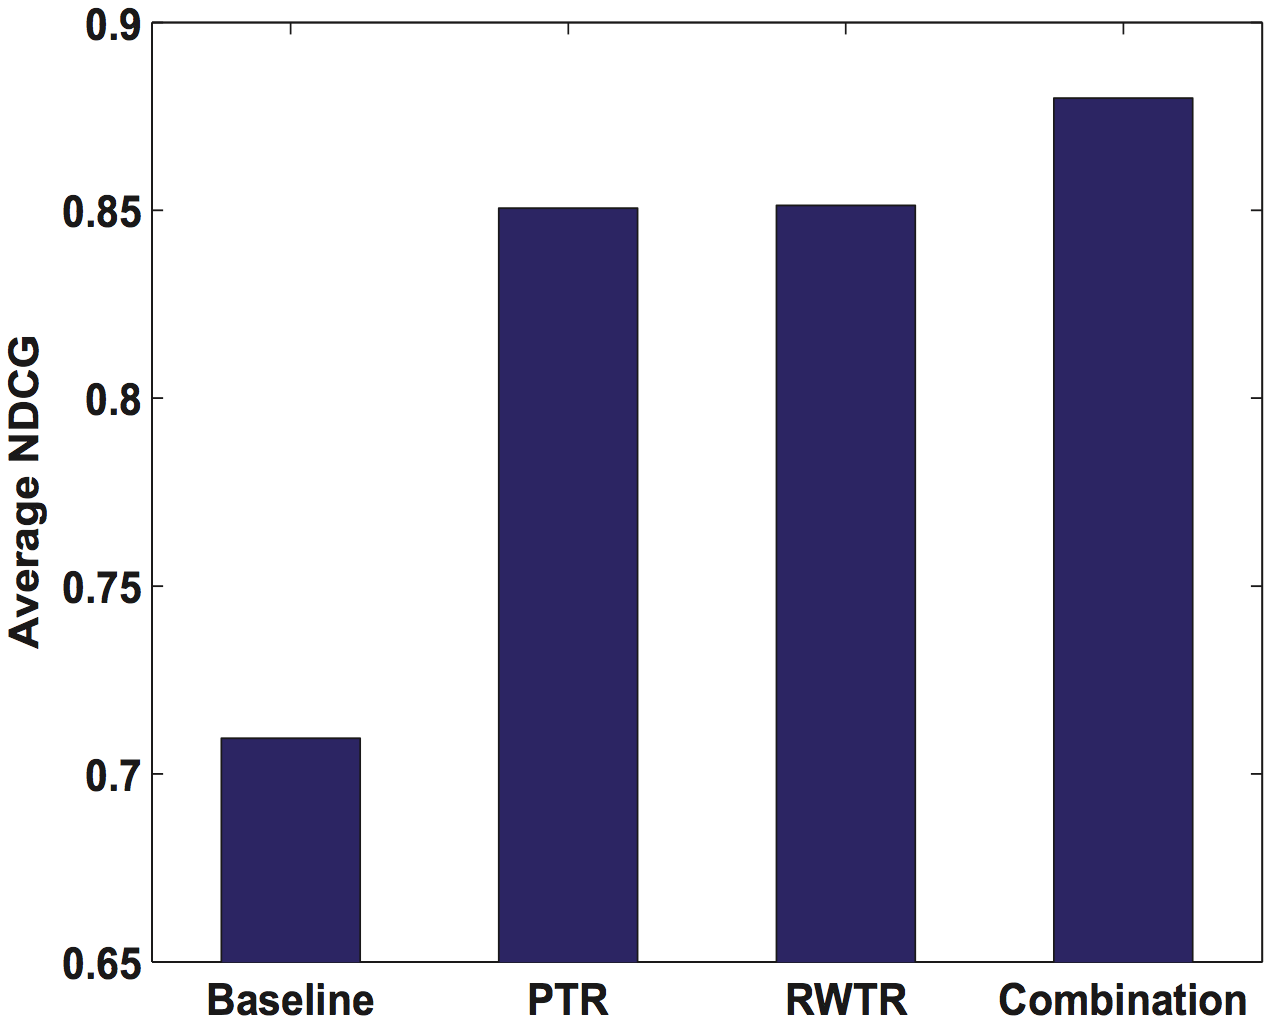
\includegraphics[height=3in]{images/ndcgAll.png}
  \caption{Messergebnisse der unterschiedlichen Tag Ranking Methoden. \emph{Baseline} ist der Wert für die Flickr Tag Liste. \emph{PTR} bezeichnet die stochastische Schätzung, \emph{RWTR} die Random Walk Ranking Methode. \emph{Combination} ist die Kombination beider Methoden.}
  \label{fig:images_ndcgAll}
\end{figure}

An der Grafik erkennt man gut, dass bereits die Tag Liste von Flickr die Tags nach ihrer Relevanz sortiert enthält, die vorgestellten Methoden nach \cite{ranking} jedoch signifikante Verbesserung mit sich bringen. Dabei ist die Kombination von stochastischer Schätzung und dem Random Walk die beste Alternative. Hierbei wird ein NDCG Wert von ca. 0,88 erreicht, was einer sehr hohen Relevanz der Tags zum Photo entspricht.

Vergleicht man die Position des relevantesten Tags vor dem Tag Ranking in Abbildung \ref{fig:images_tag_ranking_psotion_relevant_tag} und nach der Anwendung des Verfahrens in Abbildung \ref{fig:images_positionRelevantTags}, so erkennt man, dass nun ca. 40 Prozent aller Photos ihren relevantesten Tag an erster Position haben, was eine Verbesserung um knapp 30 Prozent darstellt. Das Verfahren erzielt somit eine gute Leistung bei der Ermittlung der relevantesten Tags zu einem Photo.

\begin{figure}[htbp]
  \centering
    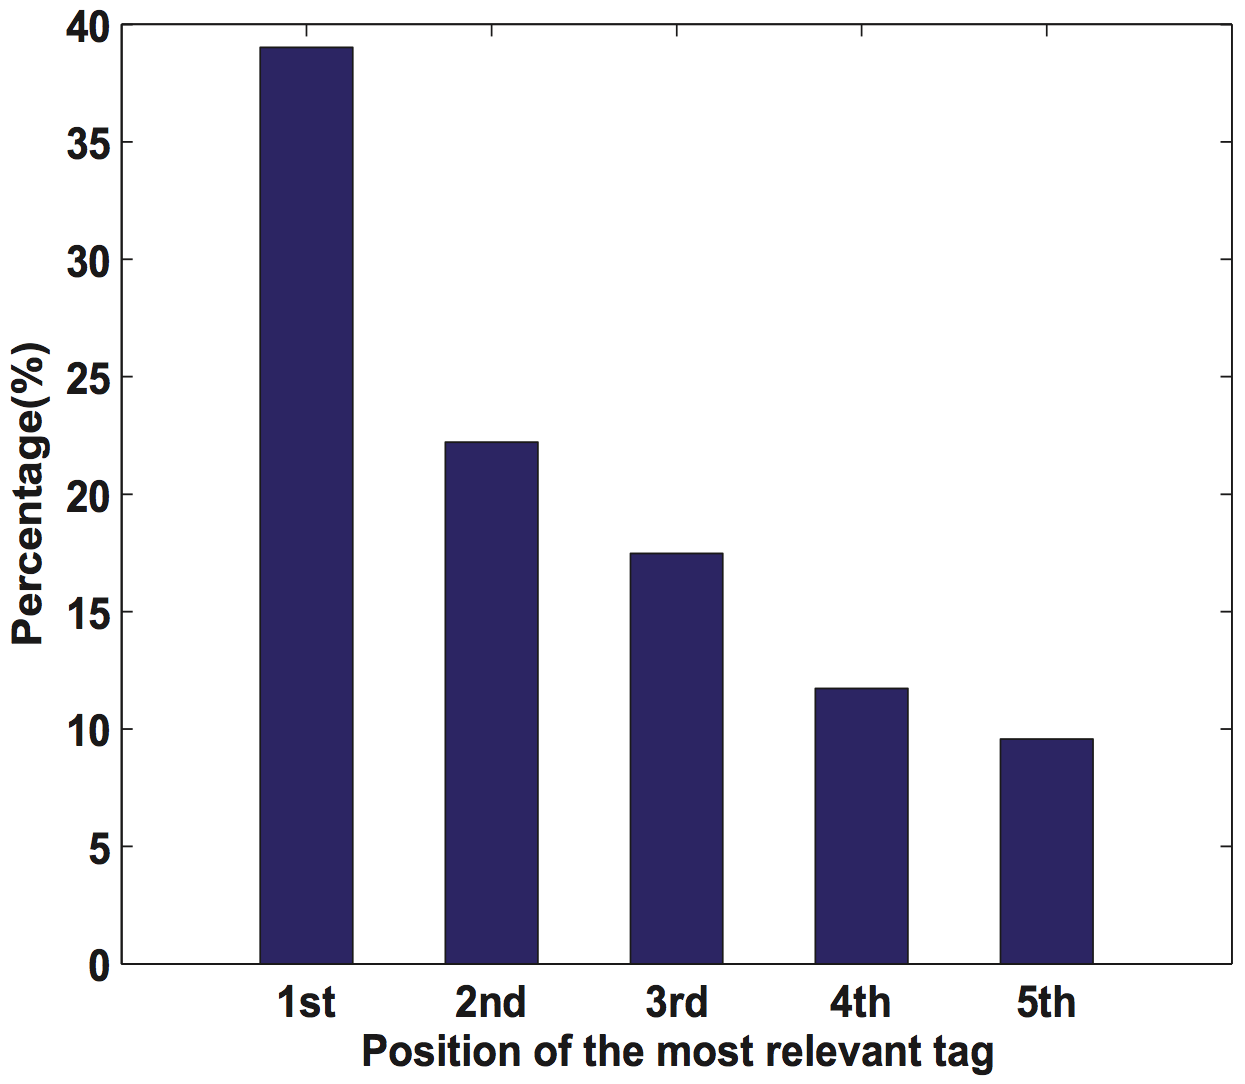
\includegraphics[height=3in]{images/positionRelevantTags.png}
  \caption{Prozentuale Anteile der Tags nach dem Ranking, die ihren relevantesten Tag an n-ter Position haben, aus \cite{ranking}.}
  \label{fig:images_positionRelevantTags}
\end{figure}


% subsubsection ergebnisse_der_evaluation_liu (end)

\subsubsection*{Zusammenfassung} % (fold)
\label{ssub:zusammenfassung_und_bewertung_liu}
Liu u. a. belegen durch die durchgeführte Evaluation eine eindeutige Verbesserung der Relevanz von Tags durch Anwendung ihres Ranking Verfahrens. Vor allem konnte eine bessere Leistung bei der Priorisierung des ersten Tags nachgewiesen werden. 

Eine Analyse der Laufzeit des Algorithmus fehlt ebenso wie Untersuchungen zur Skalierbarkeit. 


% subsubsection zusammenfassung_und_bewertung_liu (end)
% subsection ergebnisse_der_evaluation_von_ (end)

% section performance_und_skalierung (end)
